\chapter{Assignment 2: Basic Probabilities and Visualizations (2)}

\section{$\xi$ values}

\begin{itemize}
    \item $\xi_4 = 1$
    \item $\xi_5 = \frac{2}{3}$
    \item $\xi_6 = 8$
    \item $\xi_7 = \frac{1}{3}$
    \item $\xi_8 = 3$
\end{itemize}

\section{Problem statement}
\subsection*{apparition time of an owl}
Let $Y$ be the random variable with the time it takes to hear an owl (in hours).
The probability density function of $Y$ is given by:

%\begin{equation}
%    Y(t)=\xi_{5} \exp{-\xi_{6} \sqrt{t}} + \xi_{7} \exp{-\xi_{8} \sqrt[3]{t}}
%\end{equation}

\subsection*{event probability}

From $Y(t)$, we can derive the probability of the event 'hearing an owl', and more precisely its probability density function $P(t)$::

\begin{equation}
    pdf_{event}(t) = \frac{d(1-P(t))}{dt}
\end{equation}

\section{probability to wait 2-4 hours to see the event}

this probability is given by substracting $Y(4)$ from $Y(2)$. The result is $0.0048$.

\begin{figure}[h]
\centering
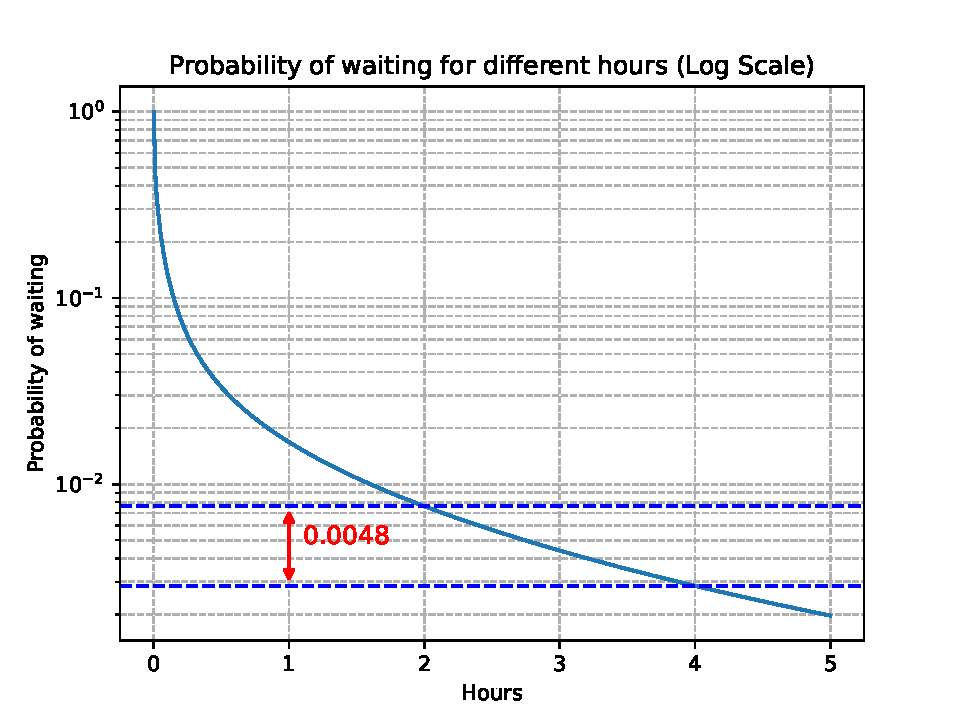
\includegraphics[width=13cm]{code/figures/prob_waiting_2_4.pdf}
\caption{the probability to wait between 2 and 4 hours is $0.0048$ \label{fig:waiting}}
\end{figure}
\FloatBarrier

\section{event probability density graph}

The graph of the probability density function of the event is given in figure~\ref{fig:waiting}.
\begin{figure}[h]
\centering
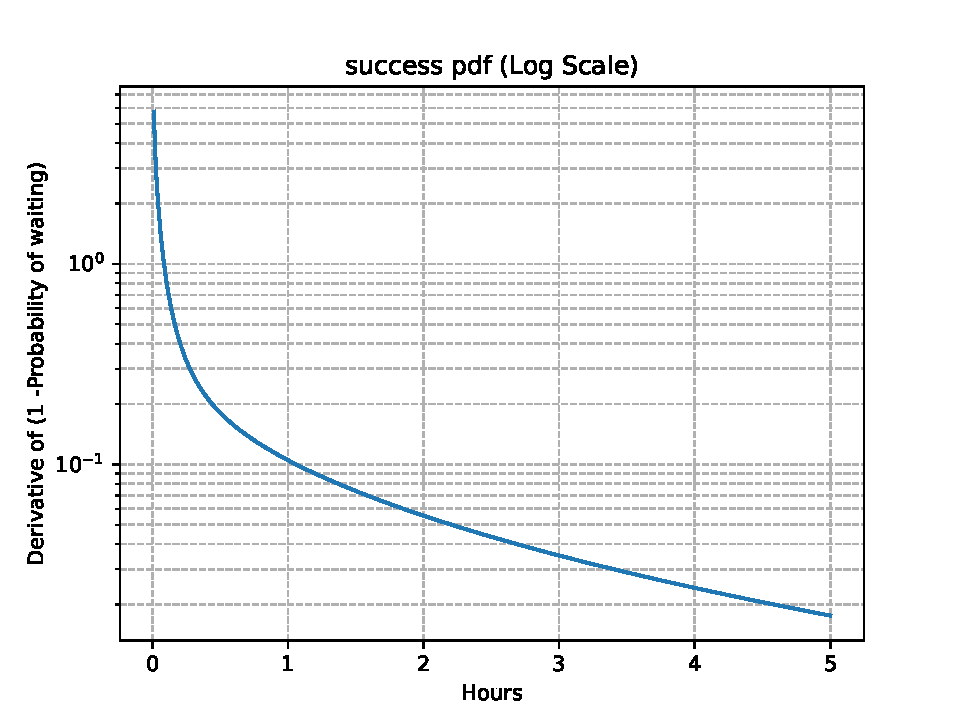
\includegraphics[width=16cm]{code/figures/waiting_time_derivative.pdf}
\caption{the probability density function of the event \label{fig:waiting}}
\end{figure}
\FloatBarrier

\section{distribution metrics}

The metrics of the distribution are given in the table below. There is a large variance, which means that the distribution is not very regular.
%make a table
\begin{table}[h]
\centering
\begin{tabular}{c|c|c}
    \hline
    metric & value & unit\\
    \hline
    mean & $5.7$ & hours \\
    variance & $1167$ & hours*hours \\
    q1 & $4.2$ & minutes \\
    q2 (median) & $30.5$ & minutes \\
    q3 & $2.5$ & hours \\
    \hline
\end{tabular}
\caption{metrics of the distribution \label{tab:metrics}}
\end{table}
\FloatBarrier

\section{distribution graph}
The graph of the distribution is given in figure~\ref{fig:distribution}.
\begin{figure}[h]
\centering
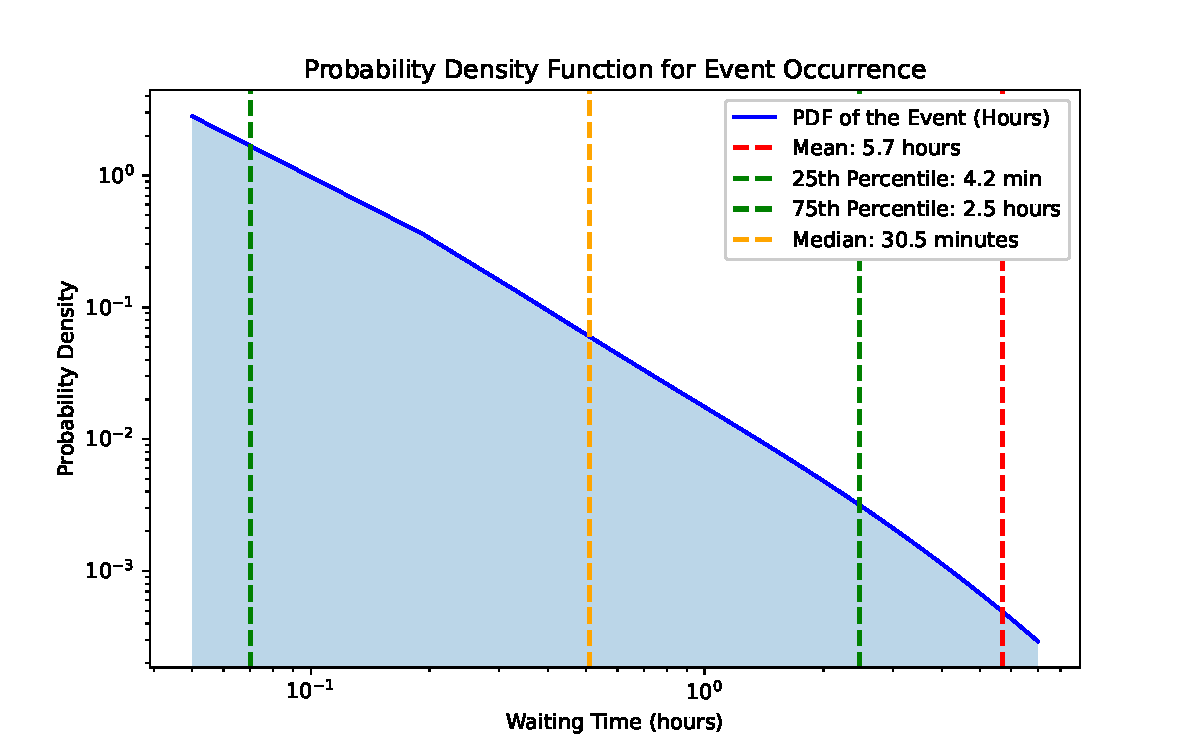
\includegraphics[width=13cm]{code/figures/pdf_event_occurrence.pdf}
\caption{the distribution of the event \label{fig:distribution}}
\end{figure}
\FloatBarrier

\section{histogram of probability of hearing the owl at given minutes (around 3 hours)}
The histogram of the probability of hearing the owl at given minutes (around 3 hours) is given in figure~\ref{fig:histogram}.
\begin{figure}[h]
\centering
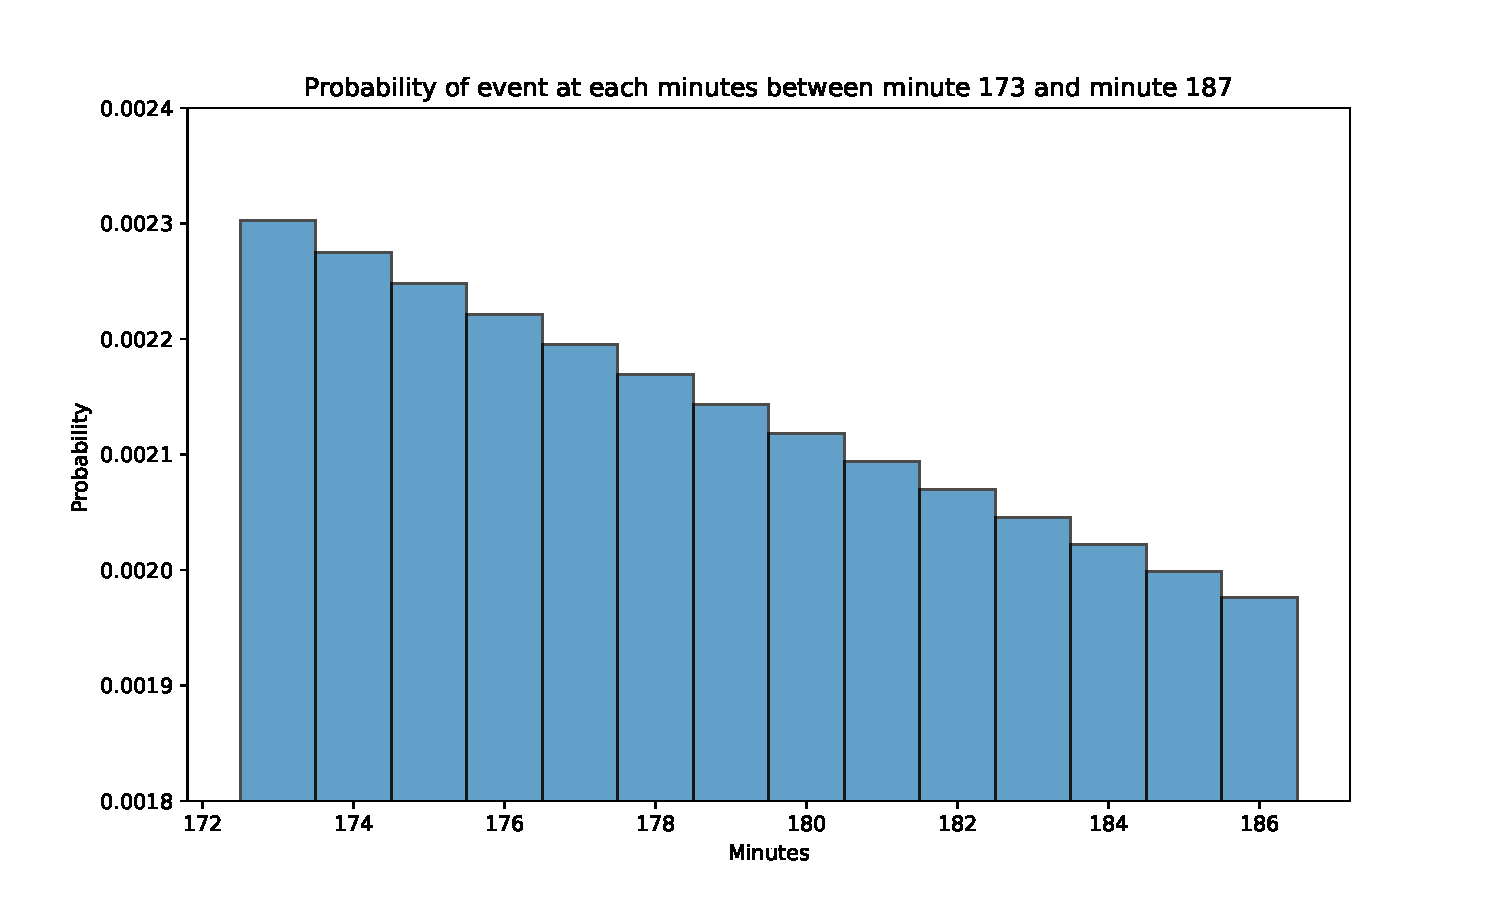
\includegraphics[width=13cm]{code/figures/event_time_dist_hist.pdf}
\caption{the histogram of the probability of hearing the owl at given minutes (around 3 hours)} \label{fig:histogram}
\end{figure}
\FloatBarrier








